\section{Planning and validation}
\label{sec:planning}

The reactive loop of \cref{sec:reactive} has two weaknesses. It has no measure of progress, and the
checks that accept its patches do not show that the weakness is gone, which the performance measure
requires. This section adds one mechanism for each weakness to \msa{} and builds both into a single
graph. It also examines the evidence on how an agent should choose its next action and on how
reliably a model can judge its own work.

A \textbf{planner} is a node that writes the steps the run intends to take into the run's state, and
revises them when the run stalls. A run \textbf{stalls} when its last three tool calls return the
same observation, the condition that the stall check of \cref{sec:reactive-stops} detects. A
\textbf{validator} is a node that decides whether to accept a patch that has passed the mechanical
checks. It is separate from the component that proposed the patch. The agent, the alert and the
tools are those of the earlier sections, so the only change is the architecture.

\subsection{What the reactive loop cannot answer about itself}
\label{sec:planning-loop-gaps}

The reactive loop records everything it has seen, but nothing in it records what the run set out to
do. As a result, the program cannot distinguish a turn that moved the run closer to an accepted patch
from a turn that only produced another observation. A turn is one pass through the loop
(\cref{sec:reactive-loop}).

The loop can detect that an observation is new. A new observation, however, does not show that the
run has moved closer to an accepted patch, so the loop has no measure of progress. The gap appears
as questions that the loop cannot answer about its own run:
\bi
\item \textbf{Is this part of the task finished?} Nothing states what finishing it would require, so
the loop cannot tell.
\item \textbf{Where is the run heading?} Halfway through a run, the trace holds the model's thoughts
so far, but none of them states where the run is heading. Neither the program nor a reader can tell
what the remaining turns are meant to achieve.
\item \textbf{What should change when part of the task proves impossible?} There is no remaining plan
to revise, because no plan was ever written.
\ei

Each question can be answered only if something was written down before the turns it asks about.
Measuring progress needs a goal to compare each turn with. Showing where the run is heading needs a
statement of intent. Changing course needs a list of remaining steps that can be replaced.

A \textbf{plan} is a list of what the run intends to achieve, written into the run's state before the
work begins. Each entry is a \textbf{plan step}. The graph in \cref{fig:planning-graph} calls plan
steps subgoals. Because the plan is in the state, the program can read it and later replace it. A
plan is the smallest addition that answers all of these questions. The model still chooses every
action, and the run gains one record that states what those actions are for.

\begin{figure*}[t]
  \centering
  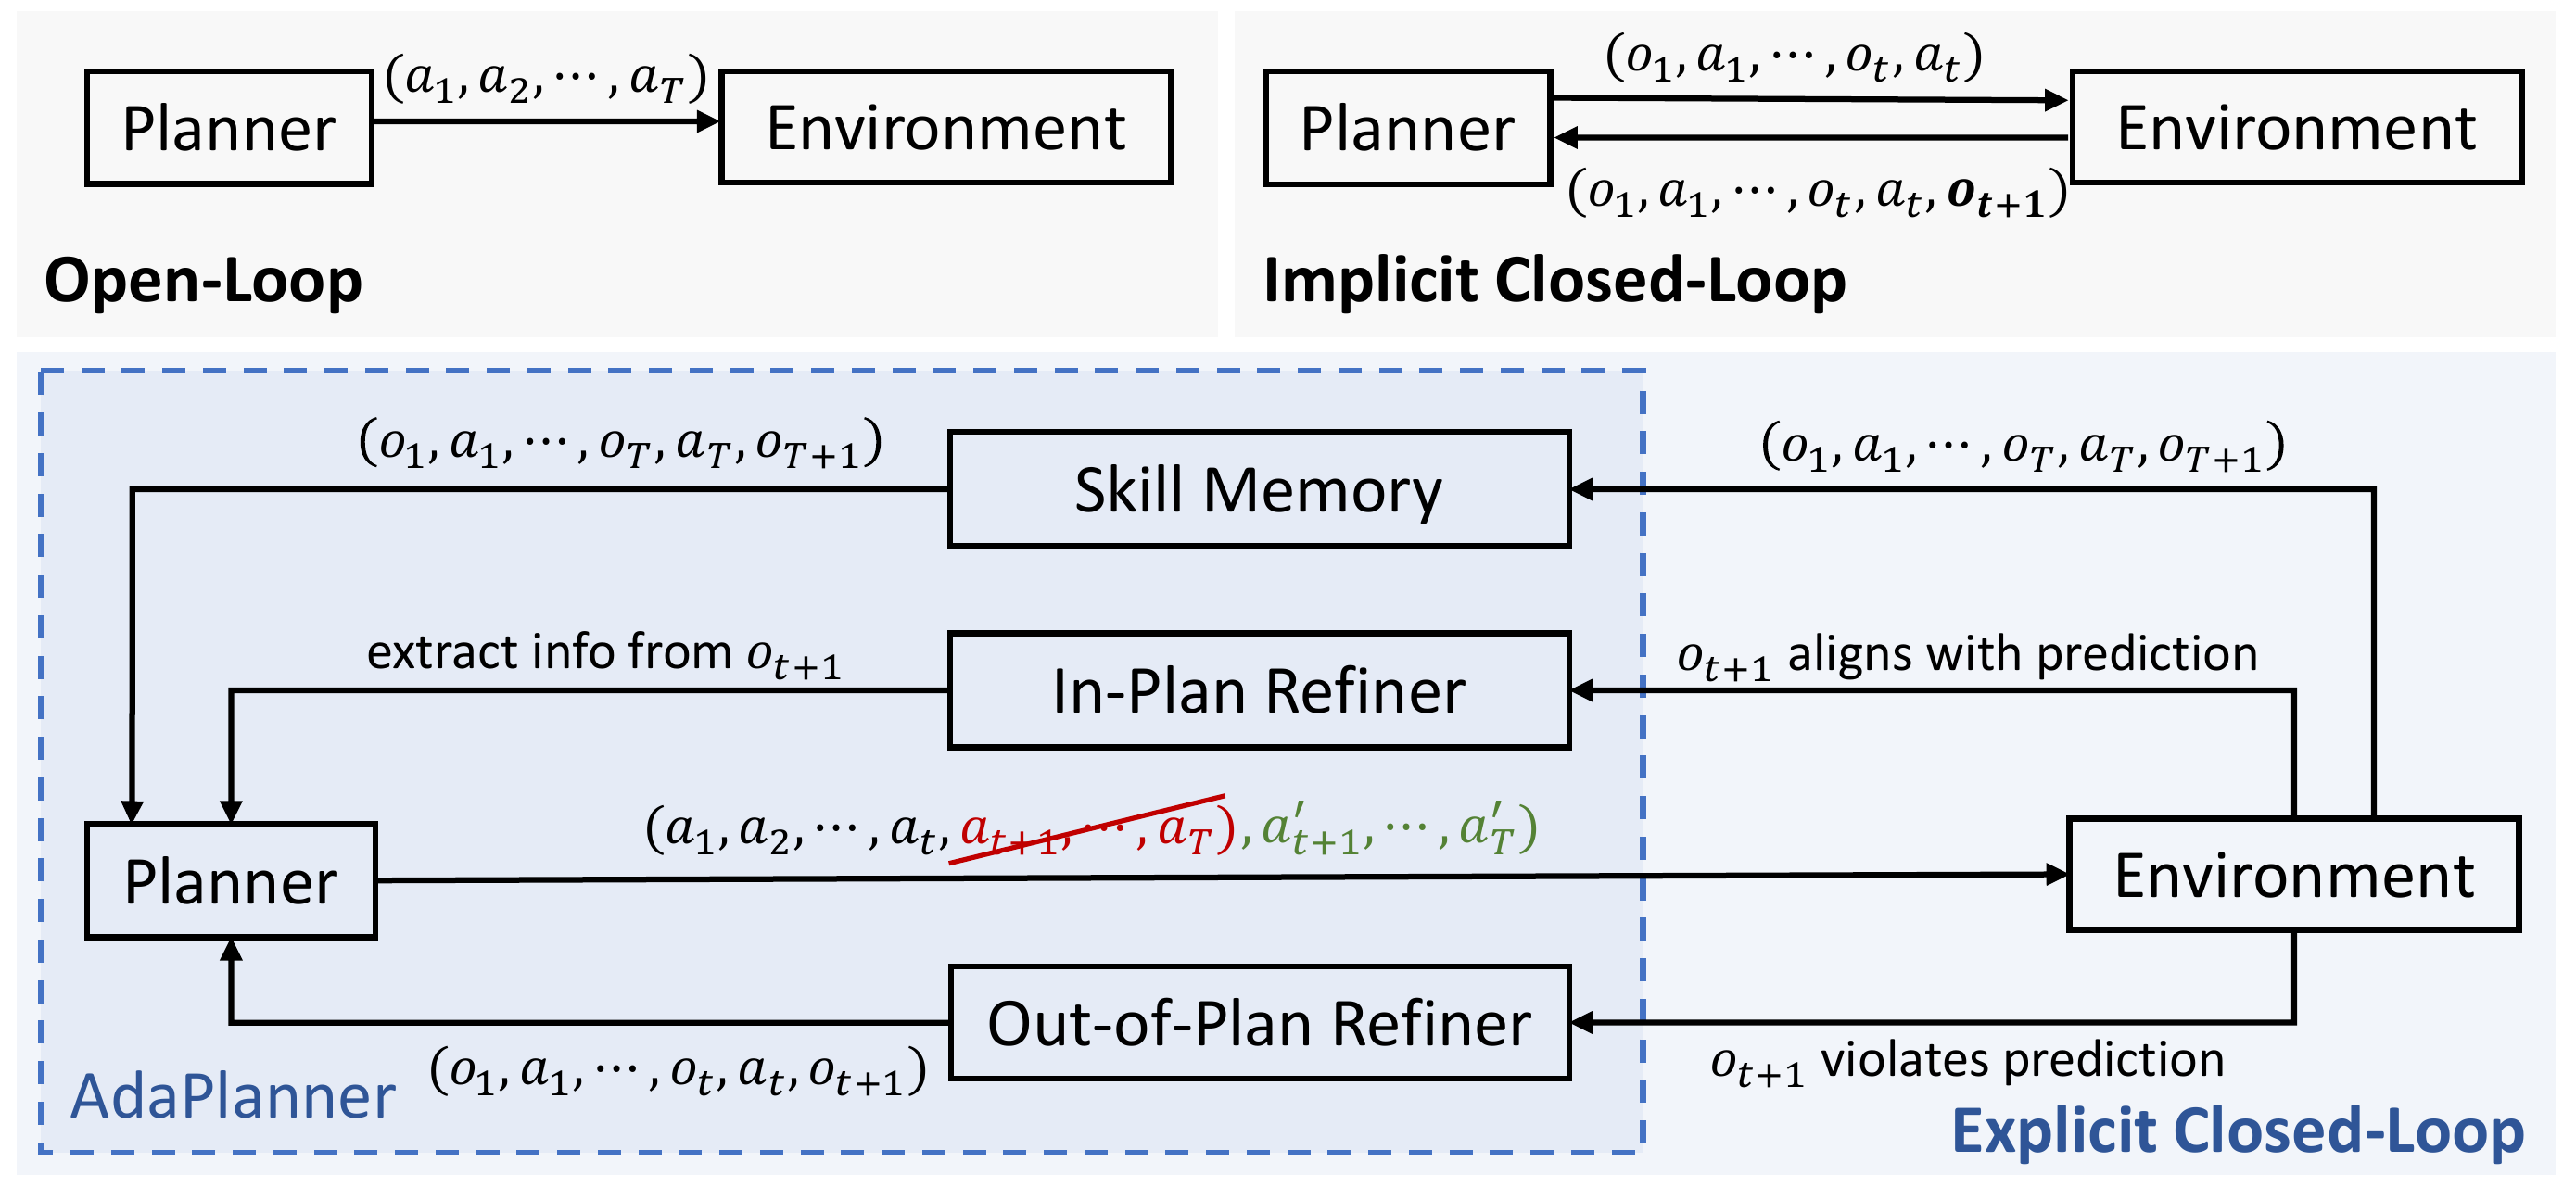
\includegraphics[width=\linewidth]{figures/adaplanner-fig1-closed-loop.png}
  \caption{Three shapes of planning: open-loop (top left), implicit closed-loop (top right) and
  explicit closed-loop (bottom), with AdaPlanner as an example of the third. Figure~1 of Sun et al.,
  AdaPlanner, NeurIPS 2023, reproduced for teaching.}
  \label{fig:planning-shapes}
\end{figure*}

\subsection{Open-loop and closed-loop planning}
\label{sec:planning-shapes}

Planners differ in how they use the observations that the environment returns after each action
\citep{sun2023adaplanner}. A planner is \textbf{closed-loop} when these observations return to it,
and \textbf{open-loop} when they do not. A closed-loop planner may use an observation only to choose
its next action, or it may use it to rewrite the rest of its plan. The open-loop planner and these
two kinds of closed-loop planner give three shapes of planning (\cref{fig:planning-shapes}).

In the figure, $a_t$ is the action taken at step $t$, $o_{t+1}$ is the observation that comes back
after it, and $T$ is the last step of the plan. The three shapes are as follows:
\bi
\item \textbf{Open-loop.} The planner sends its whole sequence of actions, $a_1$ to $a_T$, at once,
and nothing comes back. Nothing changes in response to the environment.
\item \textbf{Implicit closed-loop.} The planner sends one action at a time, and every observation
comes back to it. The plan stays as it was first written, and only the next action changes.
\item \textbf{Explicit closed-loop.} Every observation comes back, and the planner may use it to
revise the plan itself. AdaPlanner, the example in the figure, sorts each observation by whether it
agrees with what the plan predicted. When an observation violates the prediction, the planner
strikes out the remaining actions, $a_{t+1}$ to $a_T$, and writes new ones, $a'_{t+1}$ to $a'_T$, in their place.
The figure draws the struck-out actions in red and the new ones in green.
\ei

Both closed-loop shapes receive every observation. They differ in what an observation may change,
and only the explicit closed-loop shape uses it to change the plan itself.

AdaPlanner, a planning method for language-model agents, is drawn inside the dashed box as an example
of the explicit shape. It sends an observation that agrees with the prediction to an in-plan refiner,
which extracts information from the observation and leaves the plan unchanged. It sends an
observation that violates the prediction to an out-of-plan refiner, which leads the planner to
replace the rest of the plan. The skill memory in the figure is part of AdaPlanner and plays no part
in the distinction between the three shapes.

\Cref{tab:planning-shapes} summarizes the shapes. The column to compare is the last one, which says
what a planner may change when an observation arrives.

\begin{table}[htbp]
  \caption{What each shape of planning receives from the environment, and what it changes in
  response.}
  \label{tab:planning-shapes}
  \begin{adjustbox}{width=\linewidth}\begin{tabularx}{\linewidth}{L{0.3\linewidth}XX}
    \toprule
    \textbf{Planner} & \textbf{What comes back} & \textbf{What changes} \\
    \midrule
    \textbf{Open-loop} & Nothing & Nothing \\ \addlinespace
    \textbf{Implicit closed-loop} & Every observation & The next action only \\ \addlinespace
    \textbf{Explicit closed-loop} & Every observation, used to revise the plan & The rest of the
      plan \\
    \bottomrule
  \end{tabularx}\end{adjustbox}
\end{table}

Judged by what an observation may change, the reactive loop of \cref{sec:reactive} resembles an
implicit closed-loop planner without a plan. Like that planner, it receives every observation and
uses it only to choose the next action. Unlike that planner, it has no plan to keep or to revise.

The loop also only ever adds to the model's context, the messages the model reads at each call.
Every observation and every thought is appended, and nothing is removed. A plan revision works
differently. It replaces the rest of the plan held in the state, so the plan the run now follows no
longer contains the steps that were replaced.

\subsection{The graph of the planner and the validator}
\label{sec:planning-graph}

We add both mechanisms to \msa{} as one graph with five nodes (\cref{fig:planning-graph}). Two of
the nodes are new: \demoref{plan}, the planner, and \demoref{validate}, the validator. The model is
called in three nodes, \demoref{plan}, \demoref{controller} and \demoref{validate}, which the figure
draws in blue.

\begin{figure*}[t]
  \centering
  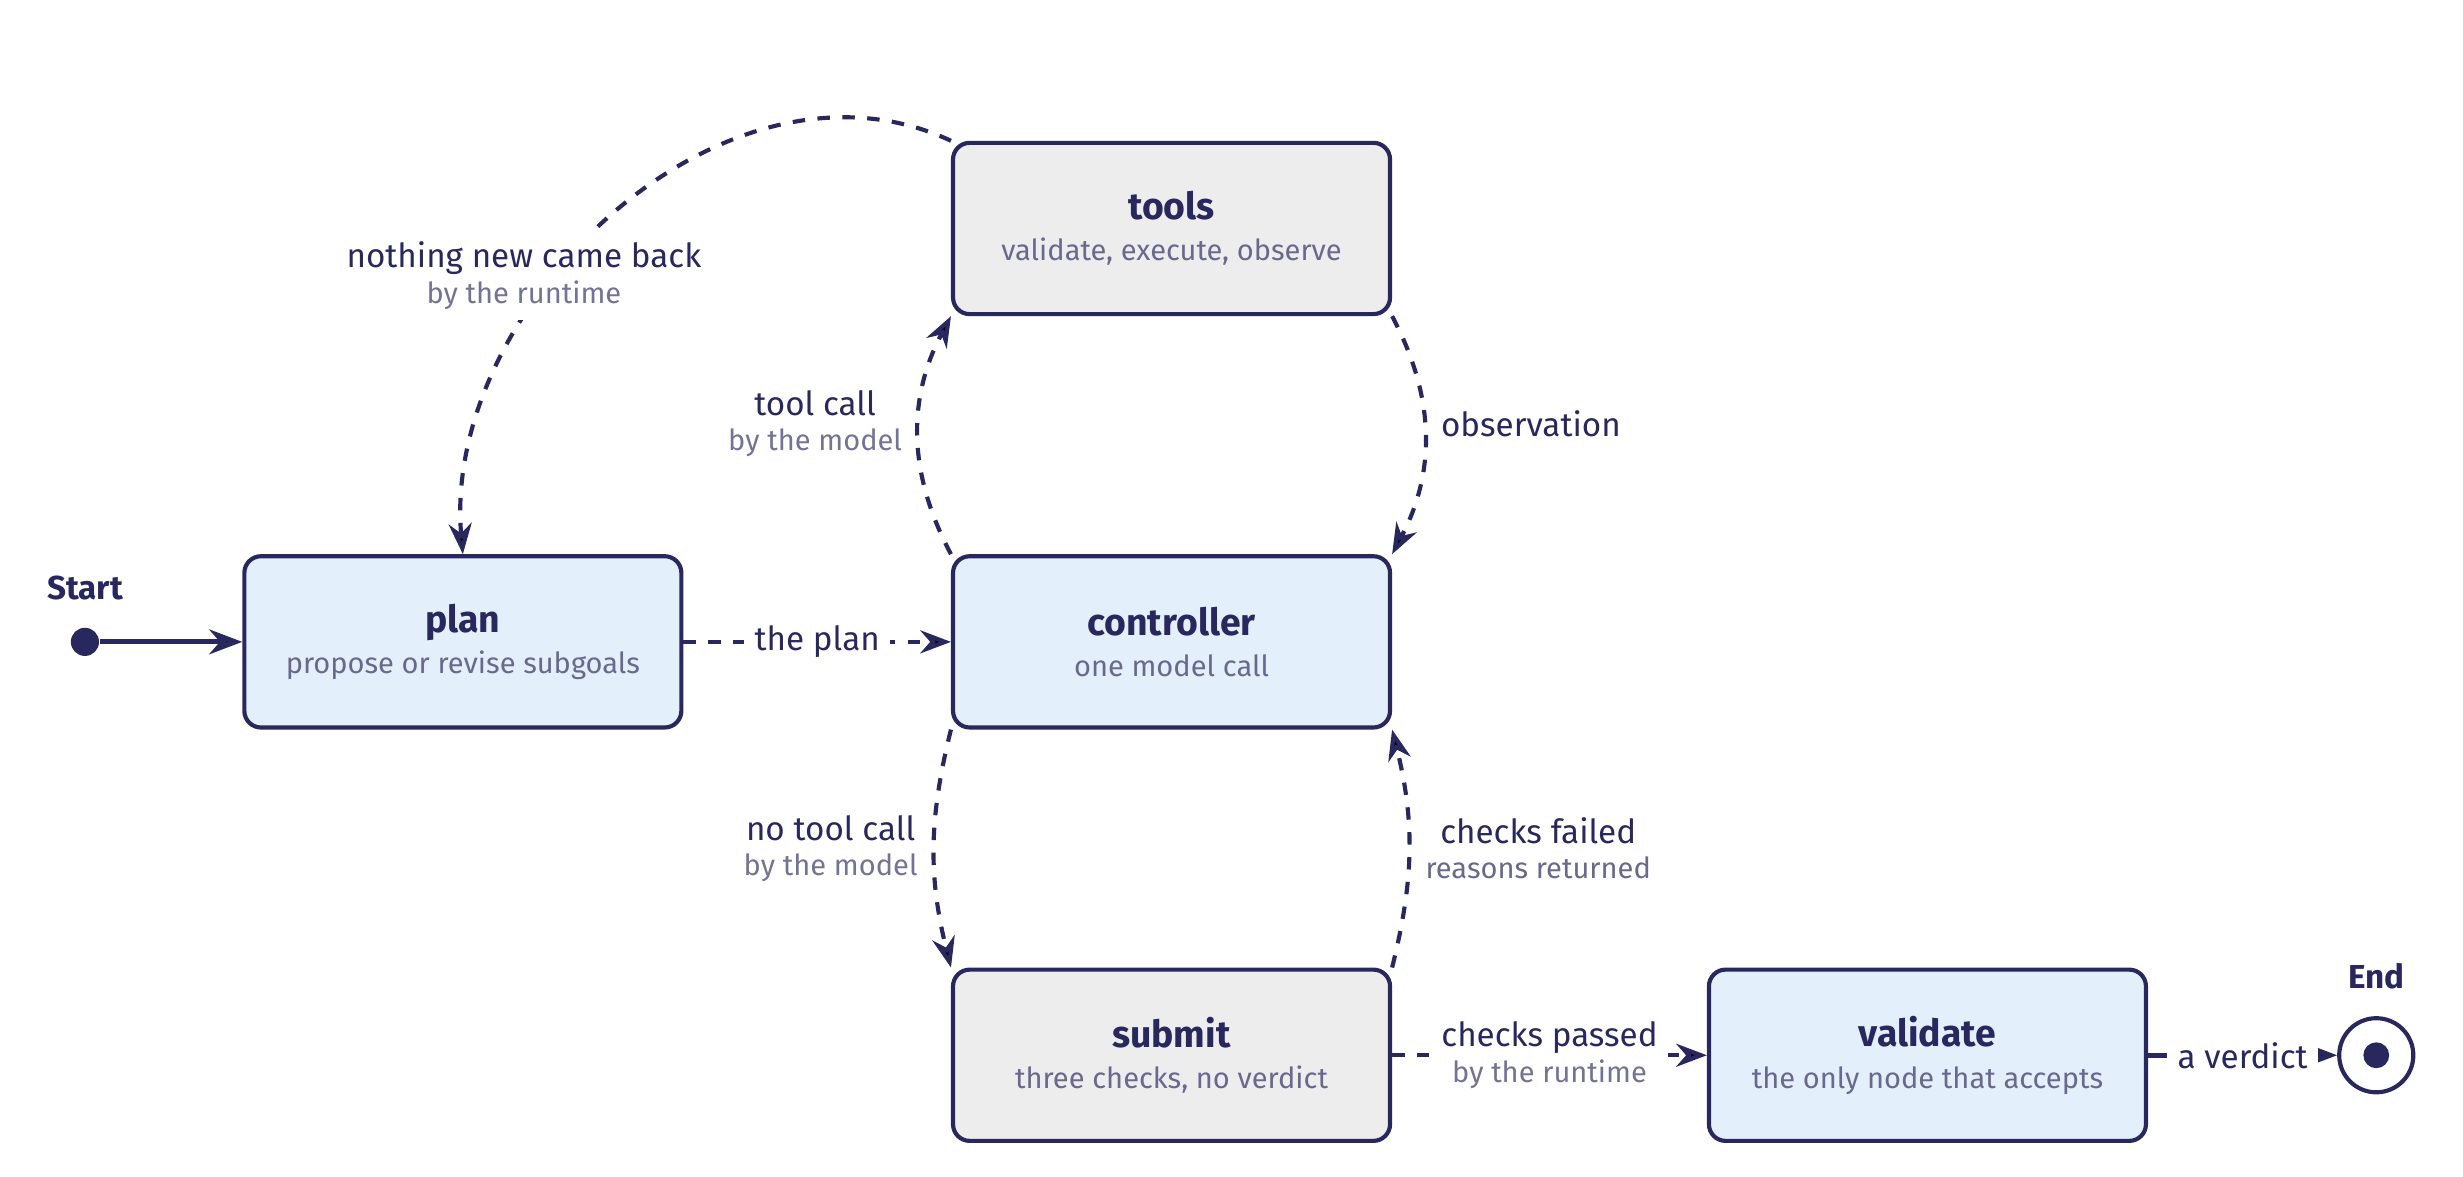
\includegraphics[width=\textwidth]{figures/deck/graph-plan-validate.png}
  \caption{The graph of the planner and the validator. Blue nodes call the model. The two solid
  edges are unconditional, and each dashed edge is one destination of a routing function we wrote.}
  \label{fig:planning-graph}
\end{figure*}

A run passes through the nodes as follows:
\bi
\item \textbf{Plan.} Every run starts at \demoref{plan}. The planner writes a plan at the start of
the run and revises it after a stall, then passes the run to the controller.
\item \textbf{Controller.} The \demoref{controller} node makes one model call. If the reply contains
a tool call, the run goes to \demoref{tools}. If it contains none, the run goes to \demoref{submit}.
\item \textbf{Tools.} The \demoref{tools} node checks the requested tool call before running it
(the dispatch step of \cref{sec:reactive-loop}), executes it and records the observation. The word ``validate'' inside this
node in the figure refers to that check of the tool call. It is unrelated to the validator. The run
then returns to the controller, or to the planner if the run has stalled.
\item \textbf{Submit.} The \demoref{submit} node runs the three mechanical checks of the reactive
loop: the patch applies, it touches the flagged line, and the rescan is clean
(\cref{sec:agents-run}). The node cannot accept the patch. If a check fails, the run returns to the
controller with the reasons. If all three pass, the run goes to \demoref{validate}.
\item \textbf{Validate.} The \demoref{validate} node is the only node that can accept a patch. Its
verdict either accepts or rejects the patch, and the run ends after the verdict in both cases.
\ei

Two edges are unconditional, which means the graph takes them every time it reaches their source.
One starts every run at the planner, and the other ends the run after the validator. They are the
solid edges in the figure. Every other edge is conditional. For each conditional edge, a routing
function that we wrote reads the state and returns the name of the next node. Each dashed edge is
one destination that such a function can return.

Two consequences follow from these edges. In the reactive loop, a run started at the controller.
With a planner, every run begins by planning, and the only way a run can end accepted is through the
validator.

A run ends without acceptance in three cases: the validator rejects the patch, the budget is
exhausted, or the run stalls a second time (\cref{sec:planning-stall}). The figure draws the first
case as the edge from \demoref{validate} to the end.

The figure does not draw the two runtime stops, the budget and the second stall. In those cases the runtime sets the run's status, and
a routing function then sends the run to its end. For the same reason, the edge from \demoref{plan}
to \demoref{controller} is dashed. Its routing function sends the run to the controller unless a stop
has already fired.

Several edges are new, but the curved edge from \demoref{tools} back to \demoref{plan}, labeled
``nothing new came back'', is the one that changes the loop itself. It is the path by which a stalled
run reaches the planner (\cref{sec:planning-tools-edge}).

\subsection{The edge from \texorpdfstring{\demoref{tools}}{tools} now has two destinations}
\label{sec:planning-tools-edge}

With a planner, the edge that leaves \demoref{tools} becomes conditional, and its second destination
is the planner. In the reactive loop, this edge was unconditional. Every observation went straight
back to the controller, which is what made the agent reactive. In code, the routing function after
the tools node looks like this:

\begin{lstlisting}[basicstyle=\ttfamily\footnotesize, caption={Routing after the tools node
(illustrative).}, label=lst:planning-after-tools]
def after_tools(state) -> str:
    if state.get("failed_step"):
        return "plan"
    return "controller"
\end{lstlisting}

The function reads one field of the state, \demoref{failed\_step}. If the field is set, the run goes
to \demoref{plan}, which revises the plan. Otherwise the run goes to \demoref{controller}, exactly as
in the reactive loop. The runtime sets the field when the run stalls for the first time
(\cref{sec:planning-stall}).

This edge changes what happens to a stalled run. In the reactive loop, a stalled run ended at once
with the status \demoref{no\_progress}. That status still exists, but a run now reaches it only after
one revision of the plan has been tried.

\subsection{How the runtime decides that the plan has failed}
\label{sec:planning-stall}

The runtime, and not the model, decides that the current plan has failed. It uses the stall check of
the reactive loop (\cref{sec:reactive-stops}): a run has stalled when three consecutive tool calls
return the same observation. The check catches one form of non-progressive iteration, the form in
which the results repeat exactly. Non-progressive iteration in other forms, and the other failure
shapes of \cref{sec:reactive-shapes}, go undetected while the run is going on.

What is new is the way a stall leads to a revision:
\bi
\item \textbf{The runtime notices.} In the reactive loop, the controller ran the stall check before
each model call and ended the run when it fired. With a planner, the \demoref{tools} node runs the
check as soon as it has recorded the new observation. When the last three results are identical, it
writes one field, \demoref{failed\_step}, instead of ending the run.
\item \textbf{The routing function reads one field.} A routing function receives the state and
returns the name of the next node. It cannot write to the state, so a judgement made inside it would
leave no record. The judgement is therefore made in the \demoref{tools} node and recorded in
\demoref{failed\_step}, and the routing function only tests whether that field is set.
\item \textbf{The planner gets one chance.} After a revision, the stall check starts counting again.
If the run stalls a second time, it ends with \demoref{no\_progress}, the same status the reactive
loop used.
\ei

Counting again needs care. The runtime only appends to the list of observations and never removes an
entry. Immediately after a revision, its last three entries are therefore still the identical results
that caused the revision. A stall check that read the whole list would count those old results
against the new plan, so the run could end before the new plan had been tried.

The runtime avoids this with a \textbf{high-water mark}, a field that records a position in a list.
The field \demoref{replanned\_at} records how many observations existed when the plan was revised.
The stall check then reads only \demoref{observations[replanned\_at:]}, the observations recorded
since the revision. The stall that caused a revision therefore cannot also count against the revised
plan.

The same field also enforces the limit of one revision. Once \demoref{replanned\_at} has been set,
the one permitted revision has been used, so the next stall ends the run instead of returning to the
planner.

Only the runtime writes \demoref{failed\_step}. The decision that a plan has failed therefore rests on
what the tools returned, rather than on the model's opinion of its own plan.

A single failed tool call is a different event from a stall, and it does not set
\demoref{failed\_step}. The runtime reissues a failed call once, without calling the model, because
a transient failure is not evidence about the plan.

In the trace, the routing event for the edge to \demoref{plan} records \demoref{by="runtime"},
because the value it tested is a field the runtime owns. As with every edge, the routing function
itself was written by us.

\subsection{What a planner changes compared with a reactive loop}
\label{sec:planning-decisions}

Adding a planner changes the answers to four questions about how a run is controlled.
\Cref{tab:planning-decisions} sets the reactive loop beside the loop with a planner, one question per
row. In each row, the last column shows what the plan adds. It gives the model's choices a scope,
records the run's intent, states what would show each step is done, and allows a second chance after
a stall.

\begin{table}[htbp]
  \caption{Questions about how a run is controlled, answered for a reactive loop and for the same
  loop with a planner.}
  \label{tab:planning-decisions}
  \begin{adjustbox}{width=\linewidth}\begin{tabularx}{\linewidth}{L{0.30\linewidth}L{0.27\linewidth}X}
    \toprule
    \textbf{Decision} & \textbf{Reactive loop} & \textbf{With a planner} \\
    \midrule
    \textbf{Who chooses the next operation?} & The model, for the whole task & The model, guided by
      the current plan step \\ \addlinespace
    \textbf{Where is the intended course recorded?} & Nowhere & In the plan, a field of the state \\
      \addlinespace
    \textbf{What would show that part of the task is done?} & Nothing is stated & The evidence named
      in the plan step \\ \addlinespace
    \textbf{What happens when the run stalls?} & The run ends & The plan is replaced, once \\
    \bottomrule
  \end{tabularx}\end{adjustbox}
\end{table}

The model still chooses the next operation, now guided by the plan step it is working on rather than
by the task as a whole. The run's intended course, which nothing recorded before, is now recorded in
the plan. Each plan step names the evidence that would show it is done. The reactive loop stated no
such condition. When the run stalls, it no longer ends at once, because the plan is replaced one time
first.

Taken together, these changes mean that the run's aim is written down before the work. The
controller's model, and anyone reading the trace, can then measure each turn against a stated goal,
rather than only against whether it produced something new. The runtime still detects a failing plan
only through the stall check, which does not read the plan (\cref{sec:planning-stall}).

\subsection{What one plan step records}
\label{sec:planning-step}

Each plan step is a small record with three fields: an \demoref{id}, a \demoref{goal} and the
\demoref{evidence}. \Cref{lst:planning-step} shows one plan step for the worked alert, as the planner
records it in the state. The flagged line of that alert is line~46.

\begin{lstlisting}[basicstyle=\ttfamily\footnotesize, caption={One plan step for the worked
alert.}, label=lst:planning-step]
{"id": 2, "goal": "read the helper the flagged line calls",
  "evidence": "the value that reaches line 46"}
\end{lstlisting}

In this step, the goal is to read the helper function that the flagged line calls. The evidence is
the value that reaches line~46, so the step is done when the run has seen which value reaches that
line. Both the fields of the record and the way the plan reaches the controller are deliberate:
\bi
\item \textbf{The goal and the evidence are separate.} The goal says what to do. The evidence says
what would show that it was done, which is the part the reactive loop had nowhere to record.
\item \textbf{The plan arrives as input.} The plan reaches the controller as a human message, that
is, a message in the role the model reads as input from a user. The plan was written by a separate
model call, the planner, and the human message records that origin. In the controller's
conversation, the plan therefore appears as an instruction the controller was given. It does not
appear among the controller's own replies, where it would look like work the controller had planned
itself.
\ei

The only tool offered to the planner's model call is \demoref{propose\_plan}, through which the
model returns the plan as a list of goals, each paired with the evidence that would show it is done.
The planner numbers the steps to give each its \demoref{id}.

If the planner's model call does not call \demoref{propose\_plan}, the planner returns no plan steps.
The run then continues without a plan, as the reactive loop would. A planner that fails to produce a
plan therefore cannot end the run. The routing after the planner sends the run to the controller
unless a stop such as the budget has already fired.

\subsection{Choosing the next action: evidence on early errors}
\label{sec:planning-wang}

\begin{table*}[t]
  \caption{Where runs go wrong under four methods of choosing the next action, aggregated over three
  benchmarks. Lower is better in the first column of numbers, and higher is better in the other
  two.}
  \label{tab:planning-wang}
  \begin{adjustbox}{width=\textwidth}\begin{tabularx}{\textwidth}{Xrrr}
    \toprule
    \textbf{How the next action is chosen} & \textbf{Dead end on move one} & \textbf{Step of first
      error} & \textbf{Recovers after it} \\
    \midrule
    \textbf{One step at a time} & 55.6\% & 1.6 & 5.4\% \\
    \textbf{Beam search} & 71.9\% & 2.0 & 11.4\% \\
    \textbf{Lookahead} & 23.6\% & 2.8 & 22.4\% \\
    \textbf{Lookahead with value propagation} & 17.8\% & 3.2 & 29.7\% \\
    \bottomrule
  \end{tabularx}\end{adjustbox}
\end{table*}

A planner looks beyond the next step. A study of action selection measured what looking ahead is
worth when an agent chooses its next action. It found that the way an agent scores its candidate
actions affects how early its runs go wrong and how often they recover
\citep[Table~3]{wang2026reasoningplan}. The study is a preprint.

The comparison changed only the method that chooses the next action and kept the rest of the agent
fixed. It was run in two agent frameworks, each held fixed, and
repeated with four language models of different sizes. The tasks were three question-answering
benchmarks. In each, an agent answers a question by taking a sequence of steps through a knowledge
graph, a database of linked facts.

All four methods pick the next action from a set of candidates. They differ in what they score each
candidate against:
\bi
\item \textbf{One step at a time.} Each candidate action is scored on its own, by how good it looks
now, and the best one is taken.
\item \textbf{Beam search.} Several of the best-scoring candidates are kept at each step instead of
one, but they are scored in the same way.
\item \textbf{Lookahead.} Each candidate is scored by the futures it leads to. The method simulates
the steps that would follow and evaluates where they end.
\item \textbf{Lookahead with value propagation.} The value of each simulated future is passed back to
the earlier choices that led to it. Evidence from late in a simulation can therefore revise a choice
made early.
\ei

A \textbf{dead end} here is an action that the researchers identified in each task in advance as a
trap: it ranks among the best by how good it looks now, but it leads the run away from good
solutions. The study reports three measures of how runs fail:
\bi
\item \textbf{Dead end on move one.} This is the share of runs whose first action is such a trap.
Lower is better.
\item \textbf{Step of first error.} This is the average step at which a run first takes a wrong
action. Higher is better, because the error comes later.
\item \textbf{Recovers after it.} This is the share of runs that recover after their first error.
Higher is better.
\ei

\Cref{tab:planning-wang} gives the results, aggregated over the three benchmarks. The rows to compare
are the first, choosing one step at a time, and the last.

Lookahead with value propagation does best on all three measures. Compared with choosing one step at
a time, it reduces dead ends on the first move from 55.6\% to 17.8\%, to about a third. It delays the
first error from step 1.6 to step 3.2, twice as far into the run. It raises recovery after the first
error from 5.4\% to 29.7\%, more than five times as often.

A \textbf{frontier model} is one of the largest and most capable models available at a given time.
The same study reports, in results not reproduced here, that a model with eight billion parameters
using lookahead with value propagation often outperforms GPT-4o, a frontier model, when GPT-4o
chooses one step at a time. In that comparison,
a better method of choosing actions made up for a much smaller model.

The evidence has limits. The tasks are question answering over a knowledge graph, not program
repair, so the numbers are not rates we should expect from our agent. Our planner also does not
simulate futures. What carries over is the pattern: scoring an action by what follows it, rather
than by how it looks now, made early errors rarer and recovery more likely.

\subsection{Why wider search does not fix myopia}
\label{sec:planning-myopia}

A score is \textbf{myopic} when it rates an action by how good it looks now, without regard to what
the action leads to. Searching more widely does not fix a myopic score. In \cref{tab:planning-wang},
beam search considers more candidates than choosing one step at a time. It does better on the step
of the first error (2.0 against 1.6) and on recovery (11.4\% against 5.4\%). Yet its first
action is a dead end more often, in 71.9\% of runs against 55.6\%.

The explanation lies in the score that each method uses:
\bi
\item \textbf{Beam search keeps the myopic score.} It ranks more candidates, but it ranks them with
the same next-step score that misled the method that chooses one step at a time.
\item \textbf{Lookahead changes the score.} What improved every measure in \cref{tab:planning-wang}
was evaluating an action by what follows it rather than by how good it looks now.
\ei

When an agent's runs go wrong early and do not recover, we should therefore first examine how it
scores its candidate actions, and only then how many candidates it considers.

\subsection{Why \texorpdfstring{\demoref{submit}}{submit} can no longer accept a patch}
\label{sec:validation}

The second mechanism added to \msa{} is the validator, the node \demoref{validate}, which decides
whether to accept a patch. It calls the model, and it is the only node that can end a run with an
accepted patch. As a result, the \demoref{submit} node can no longer accept a patch. It can only
send the patch back to the controller or pass it on to the validator.

In the reactive loop, acceptance was already separate from the controller, the component that
proposes the patch. The \demoref{submit} node accepted a patch when its three mechanical checks
passed, and no model takes part in those checks. What changes with the validator is the routing
after \demoref{submit}. In code, it looks like this:

\begin{lstlisting}[basicstyle=\ttfamily\footnotesize, caption={Routing after the submit node
(illustrative; the branch for the runtime's stops is omitted).}, label=lst:planning-after-submit]
return "validate" if checks.passed else "controller"
\end{lstlisting}

A patch that passed all three checks goes to \demoref{validate}. Every other patch goes back to
\demoref{controller}. No branch accepts the patch and ends the run, so \demoref{submit} can no longer
end a run accepted.

The checks and the validator therefore work in sequence, and they are not alternatives:
\bi
\item \textbf{The checks are a gate.} A patch that fails them never reaches the validator. It goes
back to the controller with the reasons for the failure.
\item \textbf{The validator is the only accepting exit.} It is the one node that can end a run
accepted, and every patch it sees has already passed the mechanical checks.
\ei

The validator answers a question that the checks cannot. The checks establish that the rescan is
clean. The validator is asked whether the patch is a correct fix, given that clean rescan. A clean
rescan shows that the scanner no longer recognizes the flagged pattern. It does not show that the
untrusted value can no longer reach the SQL query (\cref{sec:agents-not-rational}). Asking that second
question is the purpose of the node.

\subsection{Why the validator never reads the conversation}
\label{sec:planning-validator-inputs}

The validator is given the evidence of the run and is kept away from the conversation. The state
holds two records of what happened. The \demoref{messages} field holds the conversation with the
model, including the model's own account of what it found. We call the controller's model, which
proposed the patch, the \textbf{proposer}. The \demoref{observations} field holds what the tools
actually returned, one record per tool call, written by the runtime.

The validator's inputs are chosen accordingly:
\bi
\item \textbf{The alert, the patch and the check results.} The validator reads these. They are what
a reviewer of the patch would be given.
\item \textbf{The observations.} The validator reads what the tools returned during the run, as the
runtime recorded it.
\item \textbf{The messages.} The validator never reads this field, which holds the conversation.
\ei

The conversation is the proposer's account of the evidence, and it is kept from the validator on
purpose. A judge in court weighs the evidence itself rather than a defendant's account of it. The
validator is in the judge's position, so its verdict should rest on what the tools returned rather
than on how the proposer described it. Otherwise a confident claim in the conversation, for example
that the fix is complete, would reach the validator as if it were evidence.

Keeping the conversation away means that the validator does not read the proposer's account of its
own work. This does not make the verdict correct, because the validator is still a model judging
work.

\subsection{Self-review: accuracy and cost}
\label{sec:planning-self-review}

The validator calls a model to judge a patch, so its value depends on how reliable a model is when it
judges work. Two studies measured this. The first shows that when a model reviews and revises its own
answer without outside information, its accuracy can fall while its cost rises.

\textbf{Intrinsic self-correction} is the setting in which a model revises its answer with no
external signal. An \textbf{external signal} is information from outside the model, such as a test
result or the correct answer.

In one measurement, GPT-4 answered a benchmark of grade-school math word problems
\citep[Table~3]{huang2024selfcorrect}. Each round of self-review takes two further model calls. In
the first, the model critiques its answer. In the second, it writes a revised answer.
\Cref{tab:planning-self-review} compares no review with one and two rounds. Read the accuracy column
against the column of model calls.

\begin{table}[htbp]
  \caption{Intrinsic self-correction by GPT-4 on grade-school math word problems: accuracy and the
  number of model calls with no review, one round of self-review and two rounds.}
  \label{tab:planning-self-review}
  \begin{adjustbox}{width=\linewidth}\begin{tabularx}{\linewidth}{Xrr}
    \toprule
    \textbf{Who decides the answer is done} & \textbf{Accuracy} & \textbf{Model calls} \\
    \midrule
    \textbf{Nobody: one call, no review} & 95.5\% & 1 \\
    \textbf{The model reviews itself once} & 91.5\% & 3 \\
    \textbf{The model reviews itself twice} & 89.0\% & 5 \\
    \bottomrule
  \end{tabularx}\end{adjustbox}
\end{table}

A single call with no review answered 95.5\% of the problems correctly. One round of self-review
lowered accuracy to 91.5\% at three calls, and two rounds lowered it to 89.0\% at five calls.
Accuracy fell with each round, while the number of model calls rose to five times that of a single
answer.

An external signal changes the result. The \textbf{ground-truth label} is the known correct answer.
When the review stops as soon as the ground-truth label shows that the current answer is correct, so
that a correct answer is never revised, accuracy rises instead. A deployed agent does not have this
label at run time. If we knew the correct answer, we would not need the model to find it.

The measurement concerns one model on math problems, not program repair. It shows that, on this
benchmark, a model's review of its own work without new information made the answers worse.

\subsection{Model verifier and sound verifier}
\label{sec:planning-verifier}

A \textbf{verifier} is the component that checks a proposed answer and accepts or rejects it. Our
validator is a verifier, and so are the submit checks. A \textbf{model verifier} is a verifier that
is itself a language model, for example the model that produced the answer. A \textbf{sound
verifier}, in the sense used here, is a program that checks an answer exactly against the rules of
the task, so its verdict is always right.

Review improves results when the verifier is sound, and it can make them worse when the verifier is
the model that produced the answer. A second study compared verifiers on 100 instances in each of
several reasoning and planning domains \citep[Table~1]{stechly2025selfverification}. In each run, the
model proposes an answer and the verifier checks it. A rejected answer goes back to the model with
the verifier's critique for another attempt. Only the verifier changes between conditions. The
results below come from these domains:
\bi
\item \textbf{Graph coloring.} The task is to give each vertex of a graph one of a fixed number of
colors, the fewest the graph allows, so that no two connected vertices share a color.
\item \textbf{Game of 24.} The task is to combine four given numbers with arithmetic operations to
make 24.
\item \textbf{Blocksworld.} The task is to plan a sequence of moves that stacks and unstacks blocks
to reach a goal arrangement.
\ei

\Cref{tab:planning-verifier} gives the results for graph coloring and Game of 24. Compare each row
with the first, which is the model's first attempt without review.

\begin{table}[htbp]
  \caption{Percentage of 100 instances per domain solved correctly with no review, with review by the
  model that produced the answer, and with a sound verifier.}
  \label{tab:planning-verifier}
  \begin{adjustbox}{width=\linewidth}\begin{tabularx}{\linewidth}{Xrr}
    \toprule
    \textbf{Who decides the answer is good enough} & \textbf{Graph coloring} & \textbf{Game of 24} \\
    \midrule
    \textbf{Nobody: one attempt, no review} & 16\% & 5\% \\ \addlinespace
    \textbf{The model that produced it} & 2\% & 3\% \\ \addlinespace
    \textbf{A sound verifier} & 38\% & 36\% \\
    \bottomrule
  \end{tabularx}\end{adjustbox}
\end{table}

With the model that produced the answer as the verifier, the share of instances solved fell below
that of a single attempt: from 16\% to 2\% on graph coloring and from 5\% to 3\% on Game of 24. With
a sound verifier, the shares rose to 38\% and 36\%.

Blocksworld is the exception. There, review by the model helped, raising the result from 40\% to
55\%, and a sound verifier still did better. The exception shows that a model's critique is not
always harmful. It does not change the finding that the largest gains came from a sound verifier.

\subsection{What the studies imply for a model as verifier}
\label{sec:planning-judge}

Both studies concern puzzles and math problems, not program repair, so they give no rate we can
expect for our validator. They do support three conclusions about using a model to judge work:
\bi
\item \textbf{A model's review of its own answer is not an external signal.} When the verifier was
the model that produced the answer and it had no new information, review lowered accuracy in every
comparison above except Blocksworld. In the study that counted model calls, review also raised the
number of calls from one to as many as five.
\item \textbf{The largest gains came from information the model did not have.} Results improved most
when the procedure had the ground-truth label or a sound verifier. The one gain from self-review, on
Blocksworld, was smaller than the gain from a sound verifier.
\item \textbf{Our checks are not a sound verifier.} The rescan is a program, but it is not always
right. An edit that only renames the flagged expression can clear the alert and leave the weakness
in place.
\ei

These conclusions bear on the design of our validator. In the studies, review helped most when the
verifier had information from outside the model that produced the answer. Our validator is a separate
model call. It reads what the tools returned and the results of the checks rather than the proposer's
account of them. It also sees only patches that have already passed the mechanical checks. Neither
feature gives it a ground-truth label or a sound verifier, so neither makes its verdict always right.
The validator is a second opinion from a model, placed after checks that are cheap and reproducible
but not sound.

The planner and the validator are two of many agent architectures. \Cref{sec:patterns} examines
others, drawn from a catalogue of design patterns.

\subsection*{Key points}
\bi
\item The reactive loop records what it has seen but not what it intends to do, so it cannot measure
its progress, and a plan written into the state records that intent.
\item Open-loop planning changes nothing in response to the environment, implicit closed-loop
planning changes only the next action, and explicit closed-loop planning can replace the rest of the
plan.
\item On the first stall, the runtime, never the model, writes \demoref{failed\_step}, so the run goes
to the planner for one revision, and a second stall ends the run with \demoref{no\_progress}.
\item Each plan step records a goal and the evidence that would show it is done, and the plan reaches
the controller as a human message rather than as one of its own replies.
\item In one study of action selection, scoring an action by what follows it made early dead ends
rarer and recovery more likely, while wider search with the same myopic score made first-move dead
ends more frequent.
\item With a validator, the mechanical checks in \demoref{submit} become a gate, and
\demoref{validate}, which reads the evidence and never the conversation, is the only node that can
accept a patch.
\item In most measurements, a model reviewing its own answers without an external signal lowered
accuracy at higher cost, and the largest gains came from sound verifiers, which our rescan is not.
\ei
